% Chapter 1

\chapter{Introduction} % Main chapter title

\label{Chapter1} % For referencing the chapter elsewhere, use \ref{Chapter1} 

\lhead{Chapter 1. \emph{Introduction}} % This is for the header on each page - perhaps a shortened title

%----------------------------------------------------------------------------------------

\section{Introduction}

The arrival of E-commerce systems has contributed a great deal to the economy and it has also played a vital role in collecting a huge amount of transactional data in the form of online orders and web enquiries \cite{ons}. Social Media network sites are another good example for connecting people on the World Wide Web. Facebook status and Twitter tweets are there to get updates about friends and followers. Individuals can do many things on the internet, for example, paying road tax, submitting annual tax returns, sending emails to friends, using online banking, booking air tickets and so on.

On the other hand, online interaction between citizens and governments is on the rise since more people have access to the internet and to government content on the World Wide Web; all this information and these tools greatly facilitate interaction and it has changed from being unusual to very commonplace. 

It is quite clear that the world is changing as people have the knowledge and facilities to access information on the internet - the responsibility now increasingly lies with governments to facilitate their citizens via the provision of e-government services - and many governments around the globe have realised and accepted the change and are taking aggressive steps to tackle the problem (making public data available on the internet) \cite{colesca2015understanding}.

\begin{figure}[H]
\centering
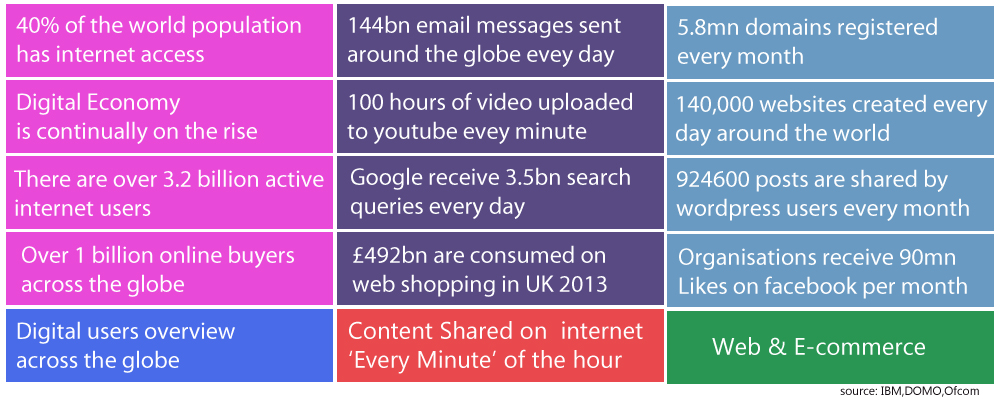
\includegraphics[scale=0.4]{chapter1/figures}
\caption{Data Facts \cite{ons}}
\end{figure}

Similarly, with such a huge volume of data, as shown in Figure 1.1, it is getting difficult day by day to analyse business and consumer behaviour. There is a greater need for analytical tools to help decision makers to understand data properly - there is no better option than information visualisation to understand and explore large amounts of data. The understanding of data will lead to the identification of trends, effective resource utilisation, educated decision making and understanding business and its core values (success and failure anticipation).

\section{Background of the Problem}

A brief summary of existing technologies in the area of research is introduced leading to the next section where the knowledge gap has been highlighted and introduced. 

Cloud based systems are gaining popularity amongst individuals, institutes and small and medium sized businesses across the globe - exploiting the Web 2.0 true potential. Web 2.0 focuses on the content which is mainly produced or created by its users \cite{3}. Similarly, data mashup systems are getting the same reception from various small and medium sized businesses on the World Wide Web \cite{patel2014enhance}. The industry leading companies such as Google, Yahoo and Microsoft are providing free cloud based services, including emails, mapping tools and cloud based storage. 

A mashup application can be characterised as a lightweight (simpler and faster) and a tactical (competitive activities) presentation layer that uses the web platform – Web-Oriented Architecture (WOA) - in order to integrate multiple sourced applications into one web-based offering \cite{4}.

Enterprise 2.0 contributes greatly to the process to generate, coordinate, collaborate and communicate content, applications and data in the business and enterprise environment. Enterprises such as small and medium sized businesses require tools which could address their core values (success and failure prediction), but also assist in decision making and providing extensive research based solutions from the existing data streams which will lead to effective resource utilisation;  not much has been done to answer these burning questions \cite{5}. 

However, information visualisation and data analysis is a field which holds the key to taking any business to the next level (expected and unexpected outcomes readiness). A business could do well and produce some quality figures in sales, but after all, it is about the techniques, how sustainable the practice is, and what further could be learned. Information visualisation converts data into interactive interfaces in order to easily understand problems, hidden patterns and scope and to explore data with a  more rapid and intuitive approach - usually abstract data are transformed into visual images to see the big picture at a glance \cite{6}.

In addressing data problems, a number of techniques \cite{7,8,9,eick1999visualizing,11} have been presented to explore data for trends, patterns and data exploration. Solutions such as pixel-oriented visualisation \cite{12} and pixel bar charts \cite{14} are available but these tools do not help with in-depth data analysis. The outstanding theoretical model which was introduced by Fry \cite{fry} is the most complete data analysis model, however the procedure is very complex and difficult to adopt without taking help from specialists on a regular basis to process data.


\section{Statement of the Problem}

The primary focus in business analytical tools or in information visualisation is on understanding data. The simple visualisation models are shown in Figure 1.2; these are basic visualisations of data included with software packages which serve basic data analysis needs. The in-depth data analysis is missing in such packages or applications. However, complex visualisation models are the outcome of research, mostly at a high level or through scientific experiments; these models provide in-depth analysis, but are very hard to practice in an enterprise environment. The main reasons are the simple visual representation, integration and compatibility issues which make it extremely hard to use the same tool for different organisations. 

\begin{figure}[H]
\centering
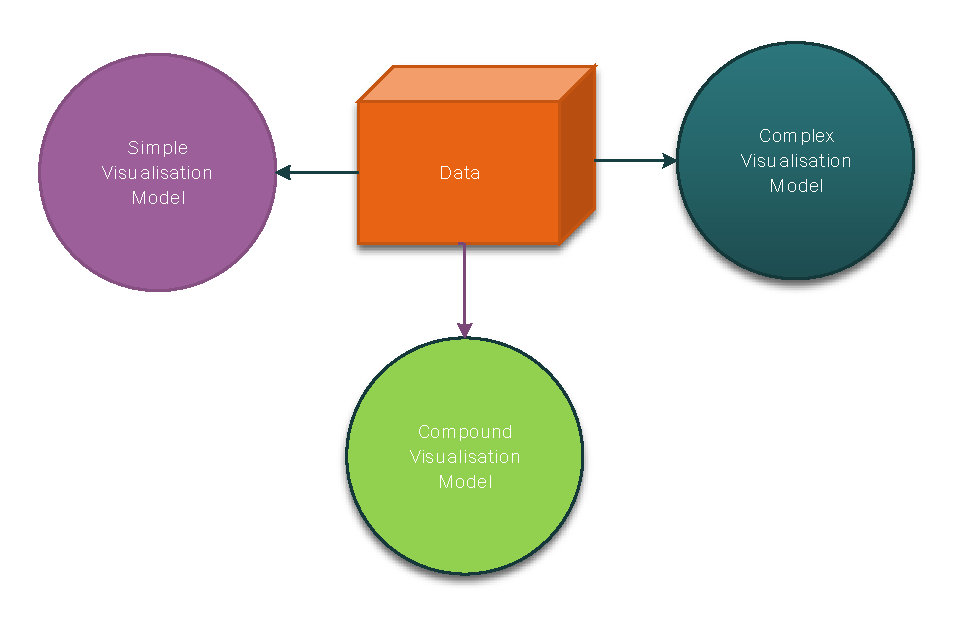
\includegraphics[scale=0.7]{chapter1/compound}
\caption{Visualisation Models Classification}
\end{figure}

However, very few visualisation models provide comprehensive solutions, but more importantly these solutions are hard to put into practice by small and medium sized businesses or individuals. There is a greater need for a compound visualisation model which is based on the concept of ease of use and integration while at the same time providing all the rich features present in complex visualisation models as there is a major knowledge gap in terms of data analysis and the human computer interaction. The research will focus on non-aggregated,  multi-attribute, multi-dimension and multi-coordinate visualisation and linked data visualisation thus making it a tremendous task and a very fresh approach in information visualisation, because the greatest contribution of information visualisation tools are to make it possible for the decision makers to identify the expected and discover the unexpected \cite{12}. Analysing complex data in a simple visualised form could be achieved through the proposed visualisation model.

\section{Purpose of the Study}

The aim of this research is to develop a data mashup system which will represent highly complex data in a simple visualised form for data analysis purposes used by businesses, individuals and government institutes. The system is targeted to reduce the technical requirements, such as data processing and data visualisation. Decision making within the system is accomplished by using a built-in pre-developed logical set of rules based on the data types and their sources. The architectural design will be so versatile that each data element could be utilised in the visualisation process upon request from the user for analysis and reporting purposes. 

\section{Objectives }

Some of the key research objectives are highlighted below.

\begin{itemize}
\item Data Analysis: 

In the recent past acquiring data was a long winded and painstaking process and one that had to be done manually. One of the main objectives of this study is to introduce an engaging and easy to use data analysis system which quickly analyses data and converts it into useful information. Data analysis and visualisation combine and form a perfect tool for the end user to understand and explore trends in large and complex data sets.

\item Information Visualisation:

Information visualisation is an act in which an individual establishes a strong connection between an internal construct and something to which access is gained through the senses. There are many types of visualisation approach introduced in the proposed system, but the following are major types which cover the unique aspects of this system and methodology. 

\item Multi-coordinate Data Visualisation:

Most software visualises data but very few display the same data in multi-coordinate views to investigate or to analyse business transactions more easily and cannot detect the failures and appreciate the accomplishments.

\item Non-Aggregated Data Visualisation:

Data visualisation practice is focused on aggregated data feeds, thus making it very difficult for the decision makers, or analysts, to find shortcomings or successes. The non-aggregated visualisation will enable users to capture unique insights about complex data in a more exhaustive analysis.

\item Multiple Attribute Data Visualisation:

The multiple attribute data techniques will visualise data with more than one data element and will help users to analyse data from different angles. This approach will help visualising multiple attribute data with coordinated visualisation for a thorough information analysis.

\item Transactional Tagging:

Tagging is widely used with social network sites, but enterprise tagging lacks research and contribution. This area needs to be investigated and business transactions need to categorise when they have successful or unsuccessful elements through data analysis and future re-use.

\item Interactivity:

Data and human computer interaction are two important aspects of any successful application. Data interaction is drilled down in the refining phase where various types of processes are applied to data to make it more meaningful for the end users. It is focused on human perspective – for example: layout, padding, proportional aspects, graph interactivity, scaling and zooming aspect of graphs for improving systems and data usability. There are many tools but a lack of user interactivity makes it very hard for businesses and individuals to get maximum usage of the systems - however the proposed system has introduced interactive and easy to use tools which give engaging overviews to the end users once the data has been processed through the data analysis phase and then visualised for the end user through data representation. The interactivity layer of the system is the bridge between the user and the application for complex analysis of data. 
\end{itemize}

\section{Significance of the Study}

This research will be a significant contribution to understanding complex data through information visualisation. The study will also be beneficial to individuals and organisations. In exploring and finding hidden trends through the high volume and complex data sets which will lead to interesting factual findings about the resources used for an activity. The significance of the subject has been divided into the following sections to give a brief overview of the research and its outcomes.

\subsection{Importance of the Study}

The data processing and storage capacity have tremendously increased; even a single transaction in a business creates many additional associated attributes. However, these attributes or data elements are not utilised directly in the business activities. The small and medium sized businesses struggle to cope with the analysis of such large amounts of data collected through various systems for the business - therefore small and medium sized businesses need a robust and easy to use and integrate visualisation system to explore and find hidden trends to help in making business decisions based on the data orientation - usage of the system is not limited to SMEs, it could be used by governmental institutes, organisations and individuals.

\subsection{Implications of the Study}

In most cases, small and medium sized businesses do not have enough resources to analyse and process collected data to explore trends and facts. The process is not easy and requires extensive data processing; however, if the collected data by any business is not analysed properly, then the actual scope of the business would be hard to identify. The comprehensive analysis of the data leads to informed decisions about the current status and provides predictions of future status - without data analysis decision making or business predictions are extremely difficult.

\subsection{Link to Existing Knowledge}

The proposed information visualisation system works closely with existing technologies such as data mashup tools for the interactivity layer and representation layer elements. The theoretical design has been derived from computational information visualisation \cite{fry} with more optimised steps both for enterprise and non-enterprise data types. The highlight of the research is based on the data representation layer, as many options are provided to the users to see visualised data in many formats and style to understand the data properly. 

\subsection{Industry Perspectives}

The visualisation model for both enterprise and non-enterprise environments brings numerous positives to small and medium sized businesses and individuals including government firms and organisations with extensive data usage. Information visualisation and data analysis bring diversified perspective about resources and outcomes. What assets of the business are bringing value to the organisations and what are the under performing assets which require attention in order to be fixed or adjusted? What are the best selling assets? What are the underselling assets? What assets require further improvements? Who are the best performers in the company or in the team? What are the current and future expected problems these assets might have? The answer to all these questions and many more bring amazing perspective to businesses and data related issues. 

\subsection{Impact on Policy Making}

Whether it is business or national policy - there are a combination of rules, plans, actions and conditions which are based on knowledge and information derived from existing techniques. All elements of policy, whether regarding its adaption or the formation of policies, are closely related to information and most of the information is generated through analysis of data through information visualisation; therefore information visualisation and data analysis play a vital role in policy making, especially for small and medium sized businesses and governmental organisations.

\section{Research Question}

The primary research question is the understanding of data through information visualisation. Enterprise 2.0 has the resources and ability to store and create a huge amount of transactional data, as Fry \cite{fry} highlighted that data and the purpose for which it was collected could be quite easily disassociated in such situations, and as a result we ask: if there is too much data, how can we understand it? 

In information retrieval systems and visualisation tools, the more specific questions users ask, the more specific and clear visualised results can be achieved, the existing techniques (\cite{7,8,9,eick1999visualizing} etc) are either developed with complex interactive and data representation or they are simple to handle complex data problems, as explained in the  problem statement above; this problem could be addressed through the compound visualisation model which gives extensive data representation to end users and the system is equipped with an interactive layer for users with no technical abilities powered by an extensive data analysis model.

For example, how many visits does a website receive? To answer this simple question, the user does not need information such as user IP address, screen resolution, browser and all the additional information stored within website statistics, but if the question is slightly changed to: how many visits does a website receive from the UK?, then users need additional information such as the IP addresses to answer such questions. Is it required to store all additional information, especially in an enterprise environment, because  users do not always know what factors are contributing towards a business success or failure. The solution does not lie with simple questions or queries but with analysing data and establishing relationships and links to data sources in visualised form.

\section{Research Design}

The concept of this research revolves around information visualisation through mashup application for enterprise and non-enterprise practice to understand huge transactional data for resource and decision making purposes, with the focus on understanding data through visualisation, interactivity of the system with the end user, storage of the generated results for re-use and comparison purposes and finally light-weight mashup applications - resource friendly and economical to run and operate. The theoretical model of the research is explained below and further explanations are provided in Chapter 3 (Research Design) and reference to existing tools and techniques are in Chapter 2 (Literature Review).

\section{Theoretical Framework}

The theoretical framework is based on four stages or layers starting with acquisition and data analysis to refine raw and complex data elements and generate information from them which is then passed onto the representation layer for representation of information in visualised form for end users. The interactive layer then creates the bridge between users and the system to customise or re-process information in various graphs and charts to explore data more effectively. The history layer enables users to store and explore generated reports for reference or comparison purposes. The proposed system is more extensively explained at the beginning of Chapter 3, which is further explained with experiments in Chapter 5 with UK postcode experiment while explaining with an advanced experiment on a business transactional data set in Chapter 6 and further experimentation in Chapter 7.

\section{Contributions}

The information visualisation model introduced in this research is a compact process for any size and type of data which is a major contribution in information visualisation and data analysis fields. Advanced data representation techniques are employed in Enterprise 2.0 using various data mashup technologies. New visualisation techniques have emerged from the research such as transactional tagging visualisation and linked data visualisation. The process and system is extremely useful in addressing complex data problems using an easy to interact and integrate with strategy. The contributions of the study are further discussed in Chapter 8.

\section{Further Work}

This research revolves around information and analysis through visualisation, as briefly explained in the introduction above; it produces results from complex data sets for small and medium sized businesses and individuals alike. However, like every system, there are some limitations in the data process and representation layer;  it depends on the nature of the data sets and the expected outcomes from complex and raw data sets.

The ability of the Visualixer system to process unstructured complex data for visualisation is a constraint as the system currently processes semi-structural data in a non-enterprise environment - the environment where data structure is not in a known state. However, the proposed system serves its purpose in an enterprise environment with the scope for improvement in data selection and versatility. The representation layer could further improve through more interactive graphs being added to the library. On-demand information, analysis and visualisation in a non-enterprise environment for non-relational data are usually not easy to represent in visual form. This could be addressed with further work and development. The mobile application of the non-enterprise visualiser will give freedom for mobile users, as mobile application usage is increasing tremendously. The non-enterprise visualiser is a cloud based system but added responsive features will add more value and will target a broader audience across different platforms. Further work and scope are highlighted in the final chapter of the thesis.

\section{Summary}

The overall structure of the thesis is highlighted in this chapter, the focus being mainly on the research problem and its background with suggestions for potential solutions and initial system design; it also gives a brief overview of the research and outlined objectives and research contributions.

There are two extensive experiments in Chapters 5 and 6 - both experiments have analysed quite large sized data sets: one from Royal Mail postcode analysis; the other was an enterprise data set with data from various different departments, along with further experimentation, in Chapter 7.

The literature review chapter gives a detailed overview of the technologies used in the research while Chapter 3 explains the theoretical framework, followed by design with system flow charts and expected outcomes while each section was being thoroughly investigated. The next chapter is the literature review; all related technologies and areas are highlighted which were used in the development and operation of this research, the focus was on data analysis and data representation along with Web 2.0 and mashup applications.



